\lecture{3}{1. September 2025}{Control volume analysis I: Basic laws and mass conservation}

\section{Basic Equations in Integral Form for a Control Volume}
In general, there are two approaches to study flowing fluids. Either one can study how an individual particle or group of particles move through space, this is often called the \textit{system approach}. This often leds to one needing to solve a set of partial differential equations.

One can also choose to study a region of space as fluid flows through it; this is the \textit{control volume} approach. This has widespread applications, e.g. in aerodynamics where the focus is often on the lift and drag on a wing rather than the individual fluid particles.

\subsection{Basic Laws for a System}
A few basic laws will be applied; these are conservation of mass, Newton's second law, the angular-momentum principle, and the first and second laws of thermodynamics. It turns out that to convert these system equations to equivalent control volume formulas we will express the properties of the system in terms of the rates of flow in and out, hence these equations are termed \textit{rate equations}.

\subsubsection{Conservation of Mass} \label{afs:consmass}
For a system we have the simple result that $M = \mathrm{constant}$. To express this law as a rate equation we write:
\[ 
\frac{\mathrm{d}M}{\mathrm{d}t} \bigg)_{\mathrm{system}} = 0
\]
where
\[ 
M_{\mathrm{system}} = \int_{M (\mathrm{system})} \, \mathrm{d}m = \int_{V \left( \mathrm{system} \right)} \rho \, \mathrm{d}V
.\]

\subsubsection{Newton's Second Law} \label{afs:N2}
For a system (the fluid) moving relative to an inertial reference frame (the control volume), Newton's second law states that the sum of all external forces acting on the system is equal to the time rate of change of the linear momentum of the system,
\[ 
\textbf{F} = \frac{\mathrm{d}\textbf{P}}{\mathrm{d}t} \bigg)_{\mathrm{system}}
\]
where the linear momentum of the system if given by
\[ 
\textbf{P}_{\mathrm{system}} = \int_{M (\mathrm{system})} \textbf{V} \, \mathrm{d}m = \int_{V (\mathrm{system})} \textbf{V} \rho \, \mathrm{d}V
.\]

\subsubsection{The Angular-Momentum Principle}
The angular-momentum principle for a system states that the rate change of angular momentum is equal to the sum of all torques acting on the system:
\[ 
\textbf{T} = \frac{\mathrm{d}\textbf{H}}{\mathrm{d}t} \bigg)_{\mathrm{system}} 
\]
where the angular momentum of the system is given by
\[ 
\textbf{H}_{M(\mathrm{system})} \textbf{r} \times \textbf{V} \, \mathrm{d}m = \int_{V(\mathrm{system})} \textbf{r} \times \textbf{V} \rho \, \mathrm{d}V
.\]
Torque can be produced both by surface and body forces and also by shafts that cross the system boundary,
\[ 
\textbf{T} = \textbf{r} \times \textbf{F}_s + \int _{M(\mathrm{system})} \textbf{r} \times \textbf{g} \, \mathrm{d}m + \textbf{T}_{\mathrm{shaft}}
.\]

\subsubsection{The First Law of Thermodynamics}
The first law of thermodynamics is a statement of conservation of energy for a system,
\[ 
\delta Q - \delta W = \mathrm{d}E
.\]
Which in rate form is
\[ 
\dot{Q} - \dot{W} = \frac{\mathrm{d}E}{\mathrm{d}t}  \bigg)_{\mathrm{system}}
\]
where the total energy of the system is
\[ 
E _{\mathrm{system}} = \int _{M(\mathrm{system})} e \, \mathrm{d}m = \int_{V(\mathrm{system})} e \rho \, \mathrm{d}V
\]
and
\[ 
e = u + \frac{V^2}{2} + gz
.\]
Here $\dot{Q}$ is positive when heat is added to the system; $\dot{W}$ is positive when work is done by the system on its surroundings; $u$ is the specific internal energy, $V$ the speed, and $z$ the height relative to a particle of substance with mass $\mathrm{d}m$.

\subsubsection{The Second Law of Thermodynamics}
When an amount of heat, $\delta Q$, is transferred to a system at temperature $T$, the second law of thermodynamics states that the change in entropy, $\mathrm{d}S$, of the system satisfies,
\[ 
\mathrm{d}S \geq \frac{\delta Q}{T}
.\]
On a rate basis this is
\[ 
\frac{\mathrm{d}S}{\mathrm{d}t} \bigg)_{\mathrm{system}} \geq \frac{1}{T} \dot{Q}
\]
where the total entropy of the system is given by
\[ 
S_{\mathrm{system}} = \int _{M(\mathrm{system})} s \, \mathrm{d}m = \int_{V (\mathrm{system})} s \rho \, \mathrm{d}V
.\]


\subsubsection{Relation of System derivatives to the control volume formulation}
Let any of the parameters $M, \textbf{P}, \textbf{H}, E,$ or $S$ be represented by the symbol $N$. Corresponding to the extensive property ($N$) that we are trying to find we, will need the intensive (i.e., per unit mass) property $\eta$. Thus:
\[ 
N_{\mathrm{system}} = \int_{M (\mathrm{system})} \eta \, \mathrm{d}m = \int_{V (\mathrm{system})} \eta \rho \, \mathrm{d}V
.\]
I.e. if:
\begin{align*}
  N &= M, & \mathrm{then} \,  \eta &= 1 \\
  N &= \textbf{P}, & \mathrm{then} \, \eta &= \textbf{V} \\
  N &= \textbf{H}, & \mathrm{then} \,  \eta &= \textbf{r} \times \textbf{V} \\
  N &= E, & \mathrm{then} \, \eta &= e \\
  N &= S, & \mathrm{then} \, \eta &= s
.\end{align*}

\subsubsection{Derivation}
\begin{figure} [ht]
  \centering
  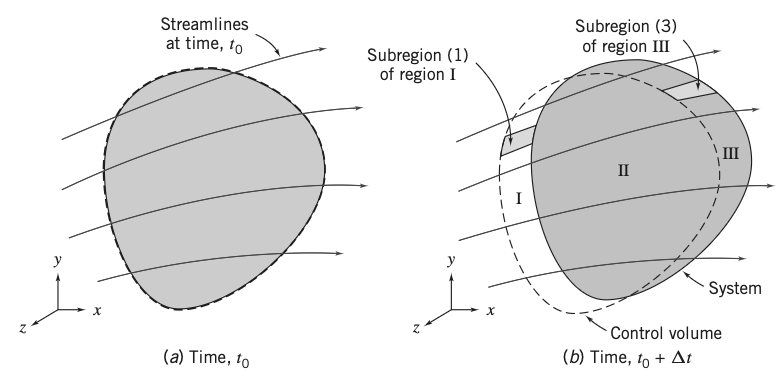
\includegraphics[width=0.5\linewidth]{./figures/f4_1.png}
  \caption{Configuration of the system and control volume.}
  \label{fig:f4_1}
\end{figure}

Let $t$ represent the initial time for the system and $t + \Delta t$ represent a small time increment later. Our objective here is to relate any arbitrary extensive property, $N$, of the system to quantities associated with the control volume. From the definition of the derivative, the rate of change of $N_{\mathrm{system}}$ is
\begin{equation}\label{eq:sysder}
  \frac{\mathrm{d}N}{\mathrm{d}t} \bigg)_{\mathrm{system}} \equiv \lim_{\Delta t \to 0} \frac{N_s )_{t_0 + \Delta t} - N_s)_{t_0}}{\Delta t}
\end{equation}
Here subscript $s$ is used to denote the system.

From the geometry of \textbf{\autoref{fig:f4_1}},
\[ 
N_s)_{t_0 + \Delta t} = \left( N_{\mathrm{II}} + N_{\mathrm{III}} \right)_{t_0 + \Delta t} = \left( N_{\mathrm{CV}} - N_{\mathrm{I}} + N_{\mathrm{III}} \right)_{t_0 + \Delta t}
\]
and
\[ 
N_s )_{t_0} = \left( N_{\mathrm{CV}} \right)_{t_0}
.\]

Substituting these into the definition of the system derivative in \textbf{\autoref{eq:sysder}} we get
\[ 
\frac{\mathrm{d}N}{\mathrm{d}t} \bigg)_{s} = \lim_{\Delta t \to 0} \frac{\left( N_{\mathrm{CV}} - N_{\mathrm{I}} + N_{\mathrm{III}} \right)_{t_0 + \Delta t} - N_{\mathrm{CV} )_{t_0}}}{\Delta t}
.\]
Which simplifies to
\[ 
  \frac{\mathrm{d}N}{\mathrm{d}t} \bigg)_s = \lim_{\Delta t \to 0} \frac{N_{\mathrm{CV}})_{t_0 + \Delta t} - N_{\mathrm{CV}})_{t_0}}{\Delta t} + \lim_{\Delta t \to 0} \frac{N_{\mathrm{III}})_{t_0 + \Delta t}}{\Delta t} - \lim_{\Delta t \to 0} \frac{N_{\mathrm{I}} )_{t_0 + \Delta t}}{\Delta t}
.\]
Each of the three terms can now be evaluated individually. We start with term 1, which simplifies to:
\[ 
\lim_{\Delta t \to 0} \frac{N_{\mathrm{CV}} )_{t_0 + \Delta t} - N_{\mathrm{CV}})_{t_0}}{\Delta t} = \frac{\partial N_{\mathrm{CV}}}{\partial t} = \frac{\partial }{\partial } \int_{\mathrm{XC}} \eta \rho \, \mathrm{d}V 
.\]

\begin{figure} [ht]
  \centering
  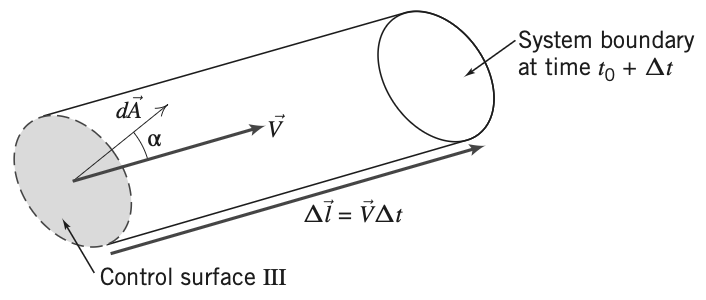
\includegraphics[width=0.5\linewidth]{./figures/f4_2.png}
  \caption{Enlarged view of subregion 3 from \textbf{\autoref{fig:f4_1}}}
  \label{fig:f4_2}
\end{figure}

To evaluate term 2 we first need develop an expression for $N_{\mathrm{III}})_{t_0 + \Delta t}$ by looking at the subregion 3 of region III shown on \textbf{\autoref{fig:f4_2}}. The vector area element $\mathrm{d}\textbf{A}$ of the control surface has magnitude $\mathrm{d}A$ and its direction is normal outward of the area element. The velocity vector $\textbf{V}$ will be at some angle $\alpha$ with respect to $\mathrm{d}\textbf{A}$

For this subregion we have
\[ 
\mathrm{d}N_{\mathrm{III}} )_{t_0 + \Delta t} = \left( \eta \rho \mathrm{d}V \right)_{t_0 + \Delta t}
.\]
To obtain an expression for the volume $\mathrm{d}V$ of this cylindrical element we first note that its vector length is given by $\Delta \textbf{l} = \textbf{V} \Delta t$. Furthermore, the volume of a prismatic cylinder, whose area $\mathrm{d}\textbf{A}$ is at an angle $\alpha$ to its length $\Delta \textbf{l}$, is given by $\mathrm{d}V = \Delta l \, \mathrm{d}A \cos \alpha = \Delta \textbf{l} \cdot \mathrm{d}\textbf{A} \Delta t$.

Then for the entire region III we can integrate and obtain the second term as:
\[ 
\lim_{\Delta t \to 0} \frac{N_{\mathrm{III}})_{t_0 + \Delta t}}{\Delta t} = \lim_{\Delta t \to 0} \frac{\int_{\mathrm{CS}_{\mathrm{III}}} \, \mathrm{d}N_{\mathrm{III}})_{t_0 + \Delta t} }{\Delta t} = \int_{\mathrm{CS}_{\mathrm{III}}} \eta \rho \textbf{V} \cdot \mathrm{d}\textbf{A}
.\]
We can perform a similar analysis for subregion 1 of region I and obtain term 3 in the equation as:
\[ 
\lim_{\Delta t \to 0} \frac{N_{\mathrm{I}} )_{t_0 + \Delta t}}{\Delta t} = - \int_{\mathrm{CS}_{\mathrm{I}}} \eta \rho \textbf{V} \cdot \mathrm{d} \textbf{A}
.\]
For subregion 1 the velocity vector acts into the control volume hence producing a negative scalar product. Hence the minus sign is needed to cancel the negative result of the scalar product.

We can now substitute in the three terms we have found as:
\[ 
\frac{\mathrm{d}N}{\mathrm{d}t} \bigg)_{\mathrm{system}} = \frac{\partial}{\partial t} \int_{\mathrm{CV}} \eta \rho \, \mathrm{d}V + \int_{\mathrm{CS}_{\mathrm{I}}} \eta \rho \mathrm{V} \cdot \mathrm{d} \textbf{A} + \int_{\mathrm{CS}_{\mathrm{III}}} \eta \rho \textbf{V} \cdot \mathrm{d} \textbf{A}
.\]
As $\mathrm{CS}_{\mathrm{I}}$ and $\mathrm{CS}_{\mathrm{III}}$ constitute the entire control surface the last two integrals can be combined as:
\begin{equation}\label{eq:reytra}
  \frac{\mathrm{d}N}{\mathrm{d}t} \bigg)_{\mathrm{system}} = \frac{\partial}{\partial t} \int_{\mathrm{CV}} \eta \rho \, \mathrm{d}V + \int_{\mathrm{CS}} \eta \rho \textbf{V} \cdot \mathrm{d} \textbf{A}
\end{equation}

\textbf{\autoref{eq:reytra}} is the fundamental relation between the rate of change of any extensive property $N$ of a system and the variations of this property associated with a control volume. This is also called the \textit{Reynolds Transport Theorem}. 

Here it is important to note that the system is defined as the matter that happens to be passing through the chosen control volume at the instant we chose. I.e.
\begin{itemize}
  \item $\frac{\mathrm{d}N}{\mathrm{d}t} \bigg)_{\mathrm{system}}$ is the rate of change of the system extensive property $N$, e.g. if $N = \textbf{P}$ we obtain the rate of change of momentum
  \item $\frac{\partial}{\partial t} \int_{\mathrm{CV}} \eta \rho \, \mathrm{d}V$ is the rate of change of $N$ in the control volume. 
  \item $\int_{\mathrm{CS}} \eta \rho \textbf{V} \cdot \mathrm{d} \textbf{A}$ is the rate at which $N$ is exiting the surface of the control volume. 
\end{itemize}

\subsection{Conservation of Mass}
We remember from \autoref{afs:consmass} that the mass of the system remains constant,
\[ 
\frac{\mathrm{d}M}{\mathrm{d}t} \bigg)_{\mathrm{system}} = 0
.\]
If we set $N = M$ and $\eta = 1$ and plug it into \autoref{eq:reytra} we obtain
\[ 
\frac{\mathrm{d}M}{\mathrm{d}t} \bigg)_{\mathrm{system}} = \frac{\partial }{\partial t} \int_{\mathrm{CV}} \rho \, \mathrm{d}V + \int_{\mathrm{CS}} \rho \textbf{V} \cdot \mathrm{d}\textbf{A} 
.\]
And combining these two gives the control volume formulation of conservation of mass:
\begin{equation} \label{eq:convolconmas}
  \frac{\partial}{\partial t} \int_{\mathrm{CV}} \rho \, \mathrm{d}V + \int_{\mathrm{CS}} \rho \textbf{V} \cdot \mathrm{d}\textbf{A} = 0
\end{equation}


\subsubsection{Special cases}
In some special cases \autoref{eq:convolconmas} can be simplified. Consider first the case of an incompressible fluid, i.e. $\rho$ is constant in space and time. Consequently \autoref{eq:convolconmas} can be written as:
\[ 
\rho \frac{\partial }{\partial t} \int_{\mathrm{CV}} \, \mathrm{d}V + \rho \int_{\mathrm{CS}} \textbf{V} \cdot \mathrm{d}A = 0
.\]
The integral of $\mathrm{d}V$ over the control volume is simply the volume, this
\[ 
\frac{\partial V}{\partial t} + \int_{\mathrm{CS}} \textbf{V} \cdot \mathrm{d}\textbf{A} = 0
.\]
For a control volume of fixed size and shape, $V = \mathrm{constant}$. The conservation of mass for incompressible flow through a fixed volume becomes:
\[ 
\int_{\mathrm{CS}} \textbf{V} \cdot \mathrm{d}\textbf{A} = 0
.\]
A useful special case is when we have uniform velocity at each inlet and exit. In this case it simplifies to
\[ 
\sum_{\mathrm{CS}} \textbf{V} \cdot \textbf{A} = 0
.\]

We now consider the case of \textit{steady}, \textit{compressible flow} through a fixed control volume. Since the flow is steady no fluid property varies with time. Consequently the first term of \autoref{eq:convolconmas} must be zero and hence for steady flow the statement of conservation of mass becomes:
\[ 
\int_{\mathrm{CS}} \rho \textbf{V} \cdot \mathrm{d}\textbf{A} = 0
.\]
When we have uniform velocity at each inlet and exit this simplifies to:
\[ 
\sum_{\mathrm{CS}} \rho \textbf{V} \cdot \textbf{A} = 0
.\]



